
\documentclass[review]{elsarticle}

\usepackage{lineno,hyperref,color}
\modulolinenumbers[5]

\journal{Nuclear Instruments and Methods B}

%%%%%%%%%%%%%%%%%%%%%%%
%% Elsevier bibliography styles
%%%%%%%%%%%%%%%%%%%%%%%
%% To change the style, put a % in front of the second line of the current style and
%% remove the % from the second line of the style you would like to use.
%%%%%%%%%%%%%%%%%%%%%%%

%% Numbered
%\bibliographystyle{model1-num-names}

%% Numbered without titles
%\bibliographystyle{model1a-num-names}

%% Harvard
%\bibliographystyle{model2-names.bst}\biboptions{authoryear}

%% Vancouver numbered
%\usepackage{numcompress}\bibliographystyle{model3-num-names}

%% Vancouver name/year
%\usepackage{numcompress}\bibliographystyle{model4-names}\biboptions{authoryear}

%% APA style
%\bibliographystyle{model5-names}\biboptions{authoryear}

%% AMA style
%\usepackage{numcompress}\bibliographystyle{model6-num-names}

\usepackage{multirow}
%% `Elsevier LaTeX' style
\bibliographystyle{elsarticle-num}
%%%%%%%%%%%%%%%%%%%%%%%

\begin{document}

\begin{frontmatter}

\title{Radiation damage of scintillator rods with different concentrations of dopants
}


%% or include affiliations in footnotes:
\author[umd]{Geng-Yuan Jeng\corref{mycorrespondingauthor}}
\cortext[mycorrespondingauthor]{Corresponding author}
\ead{Geng-Yuan.Jeng@cern.ch}
\author[umd]{A.~Belloni}
\author[umd]{Shiyuan~Duan}
\author[umd]{S.C.~Eno}
\author[umd]{T.K.~Edberg}
\author[umd]{C. Hinrich}
\author[umd]{C.~Papageorgakis}
\author[umd]{Ruhi~Perez}
\author[umd]{F. Ricci-Tam}
\author[umd]{C.~Sylber}
\author[umd]{Zishuo~Yang}
\author[umd]{Yao~Yao}
\author[umd]{Yingyue~Zhu}

\address[umd]{Dept. Physics, U. Maryland, College Park MD 30742 USA}



\begin{abstract}
The performance of plastic scintillator degrades when exposed to radiation. 
In this paper, the reduction in light output 
is studied for scintillators
with varying concentrations of the primary dopant and secondary dopant,
over a wide range of dose rates.
The scintillators used polystyrene or polyvinyltoluene as the substrate, and
produced blue or green light. \textcolor{red}{some findings here}
\end{abstract}

\begin{keyword}
organic scintillator\sep radiation hardness \sep calorimetry
\end{keyword}

\end{frontmatter}

\linenumbers

\section{Introduction}
Plastic scintillator has long been an inexpensive way to detect 
charged particles produced in particle physics experiments.  
However, its 
light output decreases with accumulated dose.  
Designers of experiments in high radiations environments expected
at future hadron colliders such as the Future Circular Collider at CERN\cite{fcc}
or the SppC in China\cite{sppc}
would benefit from an increased understanding
of radiation damage in plastic scintillators.


Plastic scintillator consist of a substrate, 
often polystyrene (PS) or polyvinyltoluene (PVT),
into which wavelength 
shifting primary and secondary dopants have been dissolved.
When a charged particle traverses the scintillator, the molecules of the substrate are excited.  
This excitation can be transferred to the primary dopant radiatively 
in the deep UV at low concentrations or 
via the F{\"o}rster mechanism~\cite{forster} at concentrations above $\approx$ 1\%~\cite{birks}.  
The primary dopant transfers the excitation radiatively to the secondary dopant.  
The visible light produced by de-excitation of the secondary flour
must traverse the scintillator to reach a photodetector, 
and can be absorbed by ``color centers'' along its path.
As the dopants are expensive, commericial scintillator typical has a 1\% concentration of the
primary dopant and a 0.1\% concentration of the secondary.

When plastic scintillator is subjected to ionizing radiation,
light self-absorption by the color centers  increases (``yellowing'') when the 
radicals created during irradiation are unterminated or 
re-terminate in ways that absorb visible light.
The transfer efficiency of the initial excitation of the polymer to the
dopants combined with the probability of 
radiative decays for the dopants (``initial light output'') can lessen
when bonds form that absorb in the ultraviolet (UV) or 
that decrease the relevent de-excitation mechanisms.

If the damage is primarily to the initial light output, increasing the concentration 
of the dopants may lessen the light reduction, as the amount of light transmitted
via the F{\"o}rster mechanism will increase, and the average path length from the primary to the
secondary will decrease.

The light output as a function of dopant concentration has been studied
at high dose rate~\cite{Bross199135}.  The authors studied light output
after a dose of 10 Mrad accumulated at a high dose rate (400 krad/hr).
They varied the concentration of the secondary dopant after optimizing the
concentration of the primary using unirradiated scintillators.  They found
the light output after irradiation did not depend on the dopant concentration.
Also, in Ref.~\cite{Majewski1989500}, the radiation resistance of 
BC-408~\footnote{Saint Gobain Corp, Les Miroirs, 18, Avenue d'Alsace, 92400 Courbevoie, France},
a blue scintillator,
was studied for different concentrations of the dopant from half to $3/2$ 
the nominal concentration.  The study was done at very high dose rate 
(36000 krad/hr) and a total dose of 3 Mrad.  
They saw that varying the concentration of the secondary dopant 
did not affect the output as studied with a $\rm{^{207}Bi}$ electron source.  
They found decreasing the secondary dopant made it less rad hard, but increasing did not help.  

In this paper, we present measurements of the light output 
of blue and green scintillator rods 
before and after irradiation for various concentrations of dopants, and
as a function of the material used for the substrate
for dose rates from \textcolor{red}{xxx to xxx}.


\section{Dose rate effects}

The effect of radiation on plastic scintillator is known to depend
both on dose and dose rate.
Two well-studied~\cite{sauli,34504,Wick1991472,289295,173180,173178,Giokaris1993315,gillen,1748-0221-11-10-T10004,clough1,bolland1,bolland2,bateman,cunliffe,Biagtan1996125}
sources of dose rate effects in plastics
involve oxygen.   The penetration depth of oxygen
during irradiation depends on the dose rate.
Where oxygen is present, peroxides, which absorb in the UV~\cite{clough1},
form almost instantaneously.  Oxygen also allows the formation
of different types of permenent color centers~\cite{clough1}.
For PS, the penetration depth goes as~\cite{Wick1991472,cloughPS}.
\begin{linenomath}
\begin{equation}
z_0^2=\frac{4 mm^2~ krad/hr}{\dot{d}}
\label{eqn:z0}
\end{equation}
\end{linenomath}
where $\dot{d}$ is the dose rate.
There is an abrupt transition between areas with and without oxygen.  The
oxygen  concentration
in the oxidized regions is almost uniform~\cite{cloughPS}.
For a tile with a thickness of 4 mm, oxygen permeates the entire sample at
a dose rate of 1 krad/hr.
For dose rates above this value, the damage to the scintillator
will depend on the dose rate, as peroxides and color centers containing oxygen will
form in this regions,
but will not in the regions without.
The rate of peroxide
formation in the areas containing oxygen can show dose rate effects as well~\cite{clough1}.
The rate of peroxide formation will scale as the
square root of  the dose rate if the bond formed is bimolecular.


\section{Sample and irradiation details}
The rods were supplied by Eljen Corporation, and
are similar to EJ-200, a blue scintillator, and EJ-260, a green one, using either
PS or PVT as the substrate.
They are rectangular, with dimensions of 1x1x5~$\rm{cm^3}$, 
and the edges were diamond milled.
The concentration of the primary dopant and the secondary dopant
was 0.5, 1.0, and 2.0 times the nominal concentration.
Fig.~\ref{fig:hd} [left] shows a photograph of some of the rods.

High dose rate irradiations \textcolor{red}{( xxx--xxx~krad/hr)}
were performed at the National Institute of Standards and Technology, Gaithersburg, MD, using their Cobalt-60 (Co-60) source.  Intermediate dose rate irradiations (\textcolor{red}{xxx--xxx~krad/hr}) were performed at Goddard Space Flight Center's Co-60 source.  Very low dose rate were measured using the GIF++ facility\cite{gif} at CERN.  The source is \textcolor{red}{Cs-137?} and the dose rate \textcolor{red}{xxx~krad/hr}.

\section{Measurement technique}
The light output from the rods is measured before and after
irradiation using an alpha source (${\rm ^{269}Pu}$), as shown in Fig.~\ref{fig:hd} [right].
Before measurement, the rods were allowed to anneal
at least 2 months,  until all the temporary damage was gone.
The rod is placed on a Hamamatsu R6091 photomultiplier tube, and the
source is placed on the rod.  An alignment jig ensures reproducibility
of the alignment of the three pieces.  The measurements were made using
a \textcolor{red}{textronics scope XXXXX}, with a charge integration
window of \textcolor{red}{xx$\mu s$}.
A typical output spectrum is shown in Fig.~\ref{fig:hd} [right].
After pedestal subtraction, the distribution is fit to a Gaussian near the peak, and its mean is used as a measure of the light yield.  The uncertainty in the light output is taken as the variation in this mean for measurements taken at different times, and after removing and replacing the rod from the jig, and is
\textcolor{red}{$\pm 2$\%}.

\begin{figure}[hbtp]
\centering
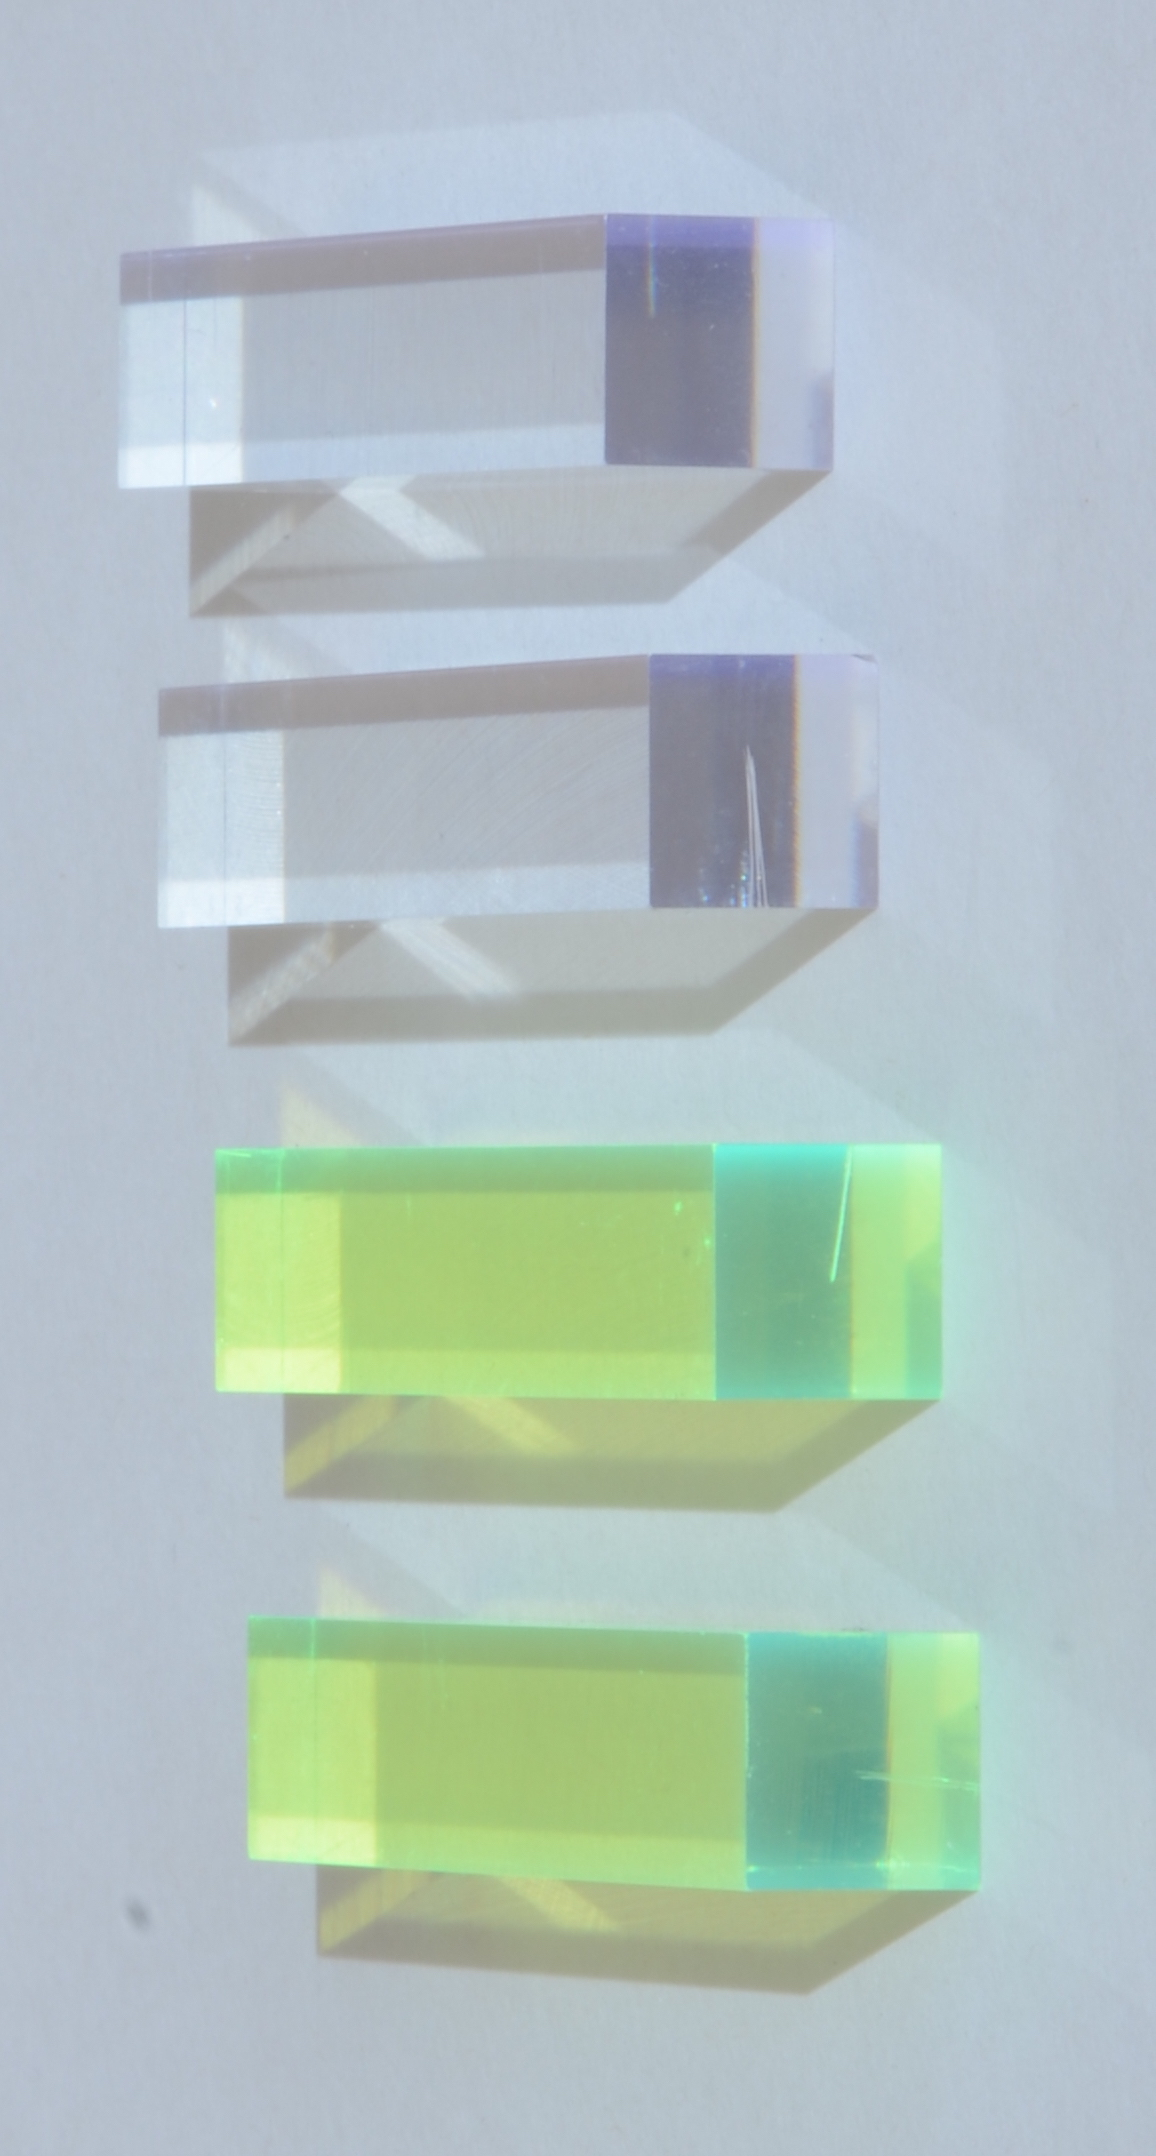
\includegraphics[width=0.32\textwidth]{photos_rods.jpg}
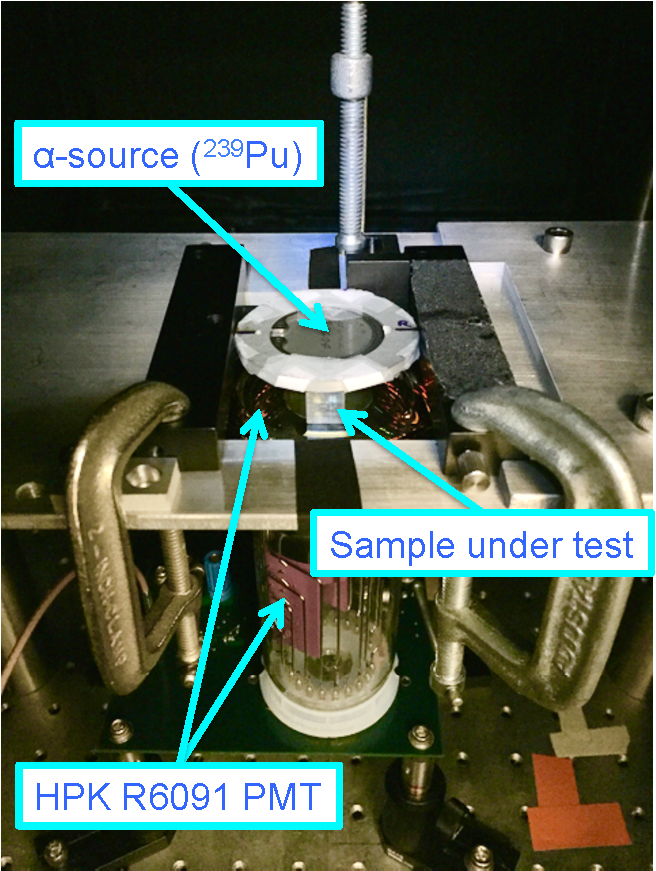
\includegraphics[width=0.45\textwidth]{Setup_AlphaSource.pdf}
\caption{
[left] photograph of some of the rods.  From top to bottom: EJ200 with nominal dopings, EJ300 with twice the nominal concentration of the primary dopant, EJ260 with nominal dopings, EJ260 with twice the nominal concentration of the primary dopant.
[right] Apparatus for measurements with alpha source.
}
  \label{fig:hd}
\end{figure}

The amount of radiation damage is quantified 
using $D$ defined in Equation~\ref{eqn:exp}.
\begin{equation}
\frac{L(d)}{L_0}=\exp{-d/D}
\label{eqn:exp}
\end{equation}
where $L(d)$ is the measured light output after a dose $d$, $L_0$ is the measured initial light
output, and $D$ is the exponential dose constant from the fit.


\section{Results}


\begin{figure}[hbtp]
\centering
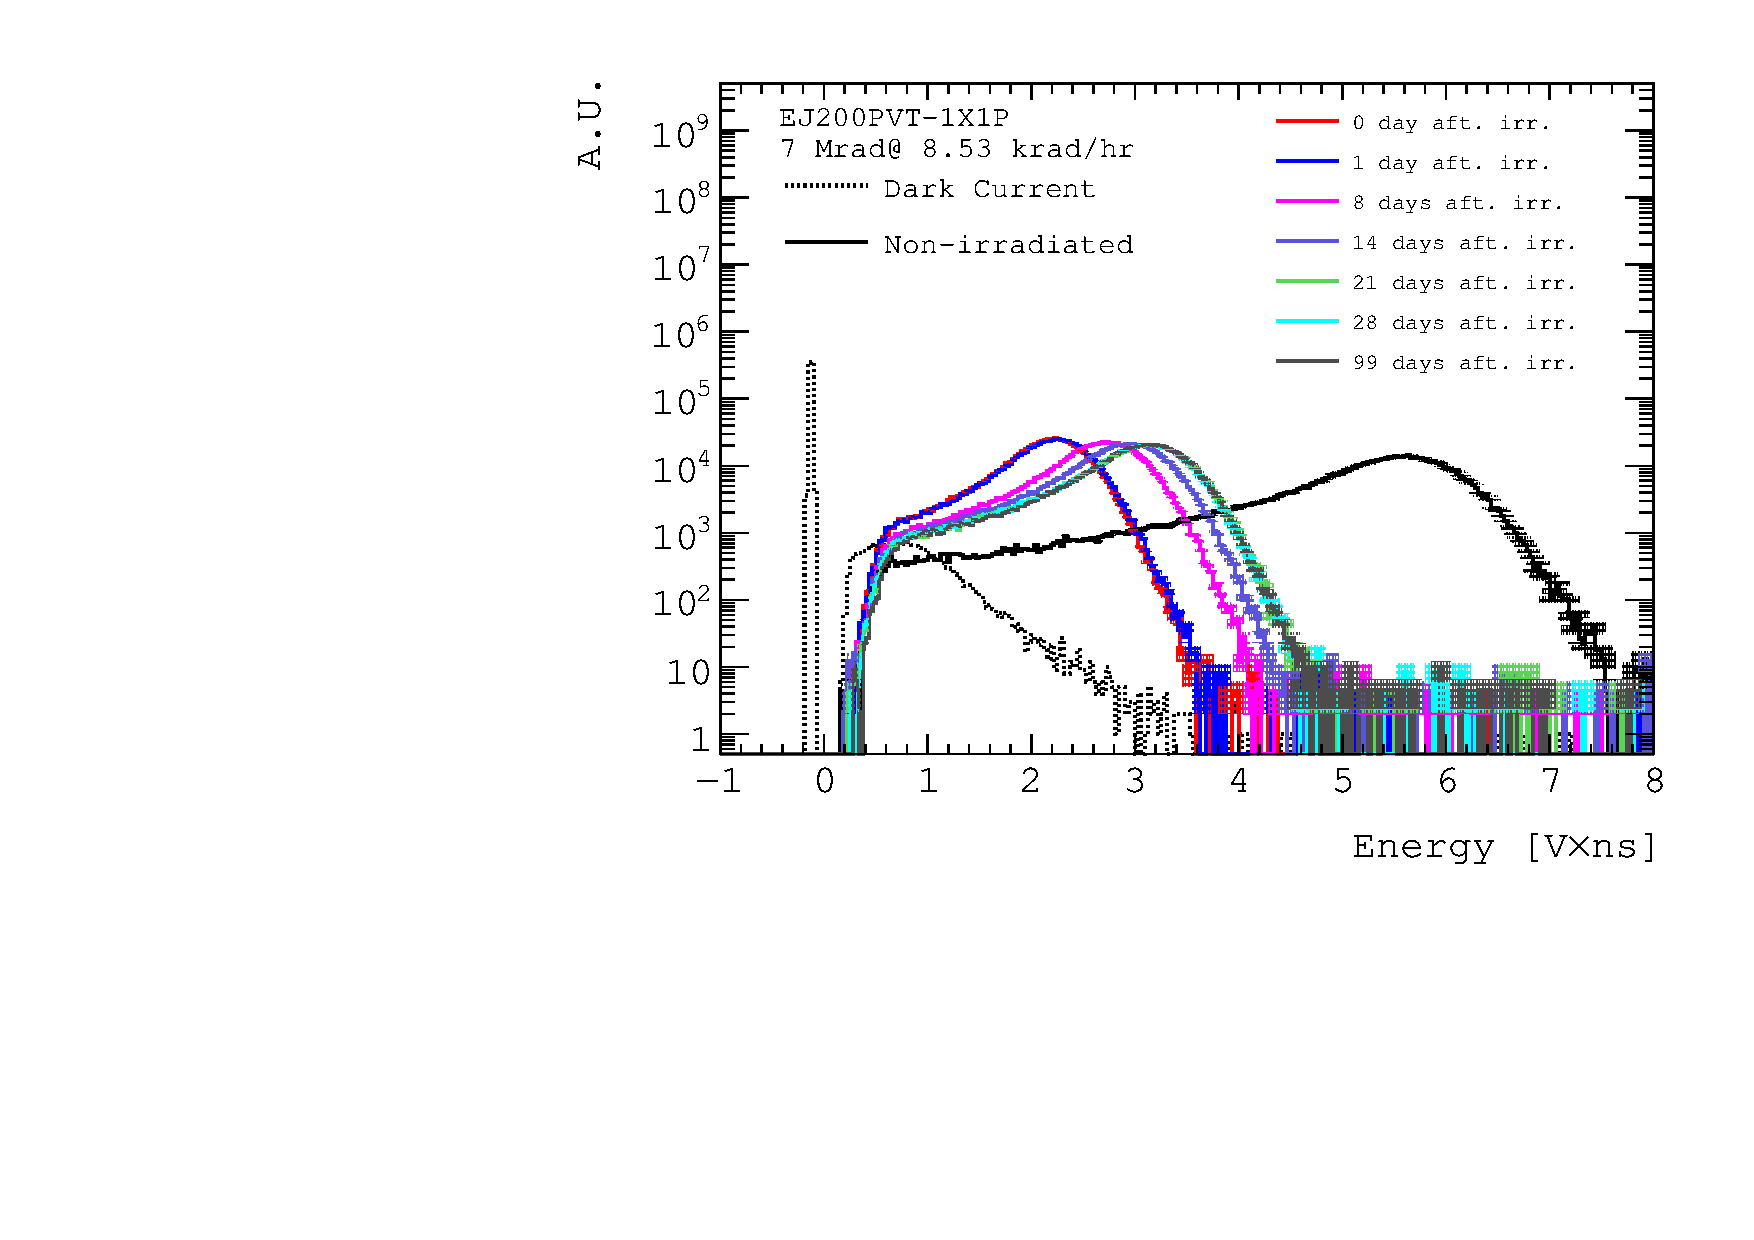
\includegraphics[width=0.45\textwidth]{figures/AlphaSourceMeasurement-EJ200PVT_1X1P_NISTRound4Set3.pdf}
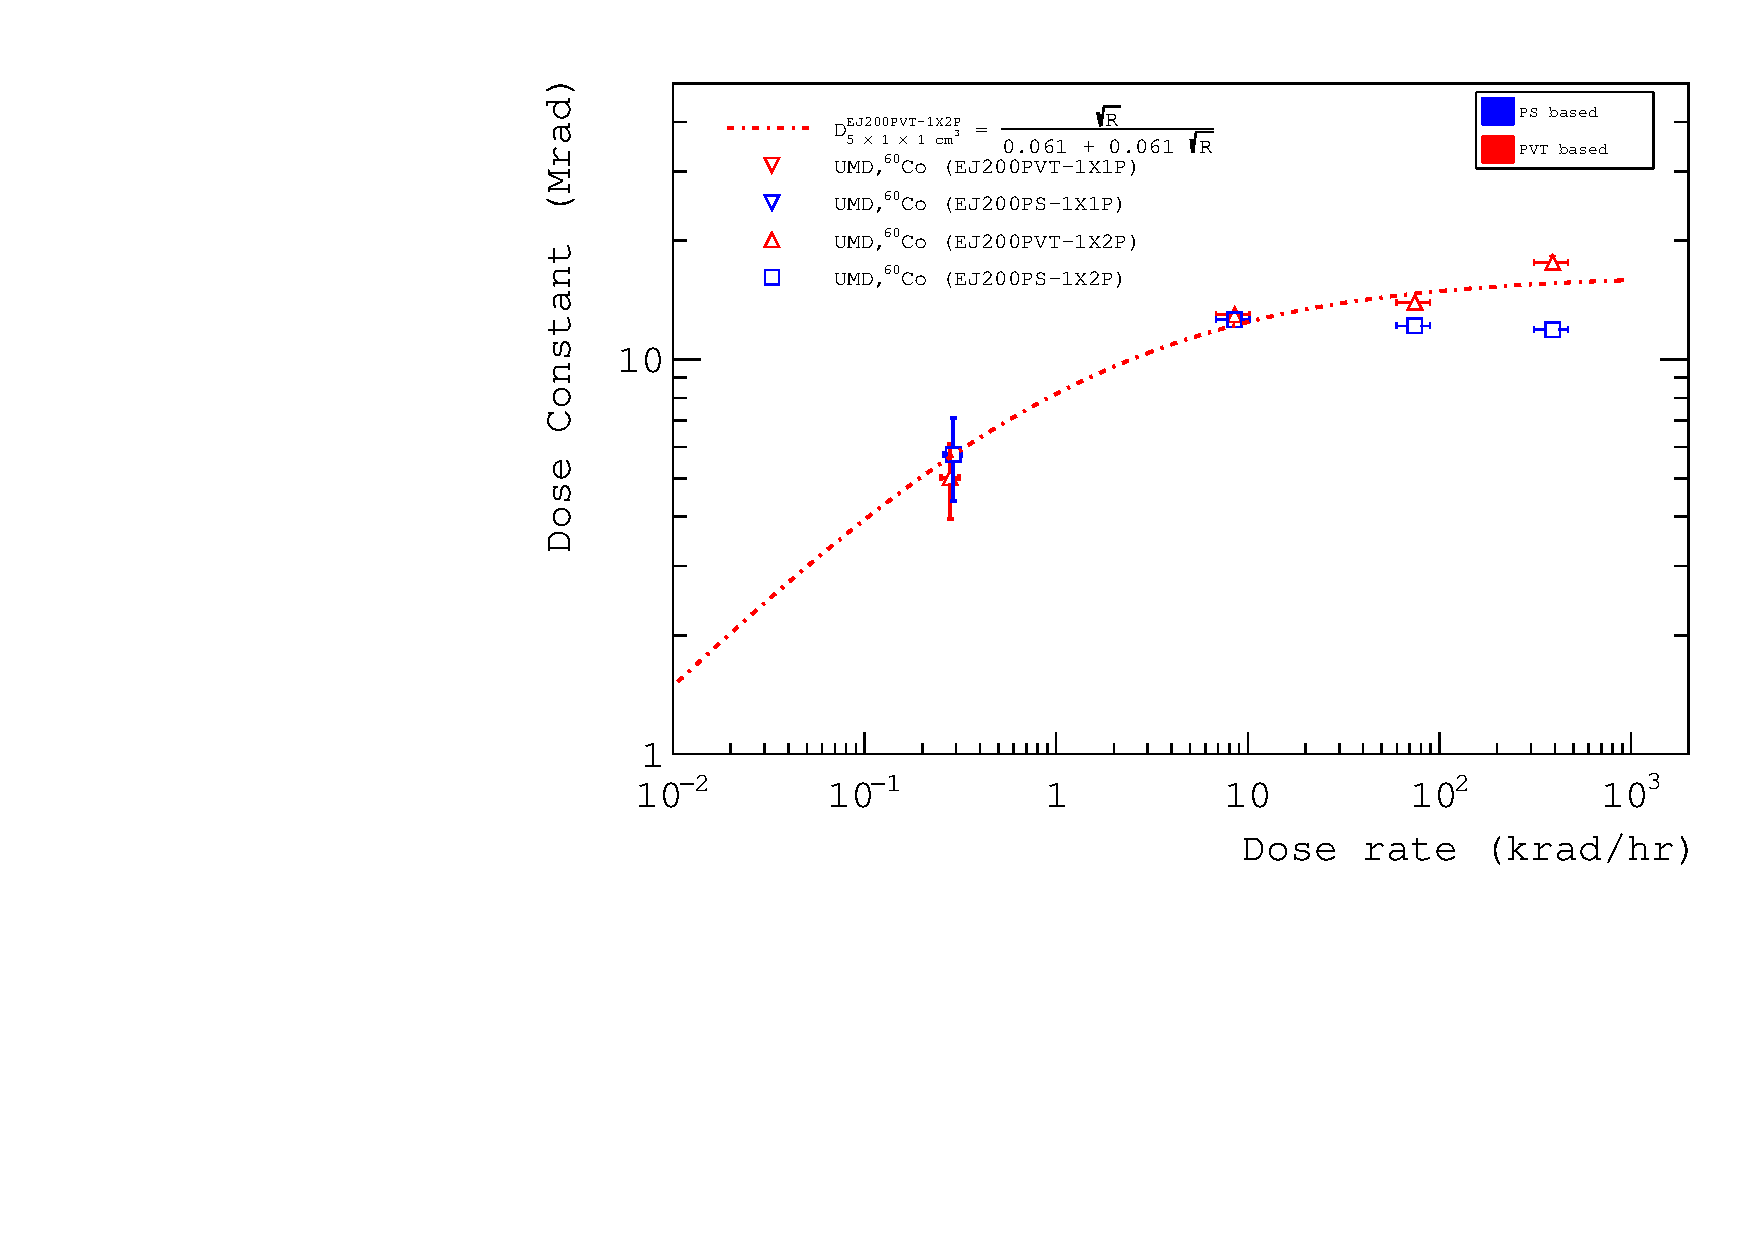
\includegraphics[width=0.45\textwidth]{figures/DoseConstVsDoseRate.pdf}
    \caption{
[left] A typical energy spectrum 
[right] resulting dose constants and comparison with the HE data. \textcolor{red}{need version without HE data}
    }
    \label{fig:GY_more2}
\end{figure}


\begin{table}[hbtp]
  \centering
  \begin{tabular}{l c l@{\hspace{1.8em}}r@{ }c@{ }l}
    \hline\hline
    Sample ID & Dose rate [krad/hr] & \multicolumn{4}{c}{Dose constant [Mrad]} \\
    \hline
%GSFC G2 (23 \deC)
    EJ-200-PS-1X2P   & \multirow{2}{*}{0.3} & & 5.75 & $\pm$ & 1.36 \\
    EJ-200-PVT-1X2P & & & 5.02 & $\pm$ & 1.08 \\
    EJ-260-PS-1X2P    & & & 5.10 & $\pm$ & 1.18 \\
    EJ-260-PVT-1X2P  & & & 5.03 & $\pm$ & 1.18 \\
    \hline
%NIST R4S3
    EJ-200-PS-1X1P   & \multirow{4}{*}{8.53} & & 12.26 & $\pm$ & 0.26 \\
    EJ-200-PS-1X2P   & & & 12.62 & $\pm$ & 0.28 \\
    EJ-200-PVT-1X1P & & & 12.46 & $\pm$ & 0.28 \\
    EJ-200-PVT-1X2P & & & 12.99 & $\pm$ & 0.30 \\
    \hline
%NIST R4S6
    EJ-200-PS-2X1P   & \multirow{4}{*}{8.34} & & 12.14 & $\pm$ & 0.23 \\
    EJ-200-PVT-2X1P & & & 13.54 & $\pm$ & 0.30 \\
    EJ-260-PS-1X1P   & & & 14.80 & $\pm$ & 0.41 \\
    EJ-260-PVT-1X2P & & & 12.53 & $\pm$ & 0.30 \\
    \hline
%NIST R4S5
    EJ-200-PS-1X1P   & \multirow{4}{*}{74.4} & & 10.63 & $\pm$ & 0.11 \\
    EJ-200-PS-1X2P   & & & 12.17 & $\pm$ & 0.15 \\
    EJ-200-PVT-1X1P & & & 13.64 & $\pm$ & 0.25 \\
    EJ-200-PVT-1X2P & & & 13.97 & $\pm$ & 0.26 \\
    \hline
%NIST R4S1
    EJ-200-PS-1X1P   & \multirow{4}{*}{390.0} & & 9.96 & $\pm$ & 0.21 \\
    EJ-200-PS-1X2P   & & & 11.90 & $\pm$ & 0.32 \\
    EJ-200-PVT-1X1P & & & 16.06 & $\pm$ & 0.57 \\
    EJ-200-PVT-1X2P & & & 17.62 & $\pm$ & 0.69 \\
    \hline
%NIST R4S2
    EJ-200-PVT-2X1P & \multirow{3}{*}{390.0} & & 16.92 & $\pm$ & 0.56 \\
    EJ-260-PS-1X1P   & & & 11.94 & $\pm$ & 0.31 \\
    EJ-260-PVT-1X2P & & & 13.92 & $\pm$ & 0.43 \\
    \hline
  \end{tabular}
  \caption{(*) Sample type, dose rate, and dose constant.  
In the naming convention EJ-XXX-YY-NXMP, XXX refers to blue (200) or green (260) scintilator, YY refers to the substrate (PS or PVT), NX refers to the 
concentration of the
secondary relative to the nominal,
and YP refers to the concenation of the primary dopant relative to the nominal.
}
  \label{tab:results}
\end{table}






\section{Conclusions}

\section{Acknowledgments}
The authors would like to thank Chuck Hurlbut of Eljen Corporation for supplying many of the rods.
The authors would like to thank the staff
Goddard Space Flight Center and at the National Institute of Standards and Technology irradiation
Facilities group for assistance
with the irradiations. 
This work was supported in part by U.S. Department of Energy Grant DESC0010072.

\section*{References}

\bibliography{atiledopings}

\end{document}
